\chapter{Dataset radiografie polmoni di pazienti affetti da Covid-19 e metadati delle radiografie}
\label{ch:Dataset}
\section{Composizione}
Il dataset usato per effettuare lo studio è stato preso da un hackaton \cite{ai} riguardante la creazione di una rete neurale in grado di apprendere 
da immagini relative a radiografie di pazienti affetti da Covid in modo da predirre la gravità della prognosi.
\\\\
La metodologia risolutiva usata è stata ispirata dal lavoro fatto da uno dei gruppi partecipanti all'hackaton, ovvero COSBI \cite{cch}.
\\\\
Dunque il dataset usato è formato da immagini raffiguranti radiografie dei polmoni, le quali tuttavia non sono omogenee. Per tale motivo 
si è dovuto effettuare un passaggio preliminare in modo da rendere le immagini tutte della stessa dimensione, ma non distorcendole.
\\\\
Oltre alle immagini sono presenti anche un insieme di metadati riguardanti lo stato in cui il paziente è entrato all'ospedale e l'anamnesi dello stesso.
Tali metadati presentano descrivono varie informazioni relative al paziente, per tale motivo sono rappresentate anche in modo diverso: esistono dati di tipo categorico, sia con più categorie che con
due sole categoria, dati che possono essere considerati come booleani e dati interi, come ad esempio l'età.
(tutte le colonne sono elencate a pagina \pageref{eterogeneo})
\clearpage
\section{Immagini delle radiografie dei pazienti}
Dando uno sguardo alla composizione del dataset si può notare come le immagini risultano avere dimensione diversa.

\begin{figure}[h]
    \centering
    \begin{subfigure}{.45\textwidth}
        \centering
        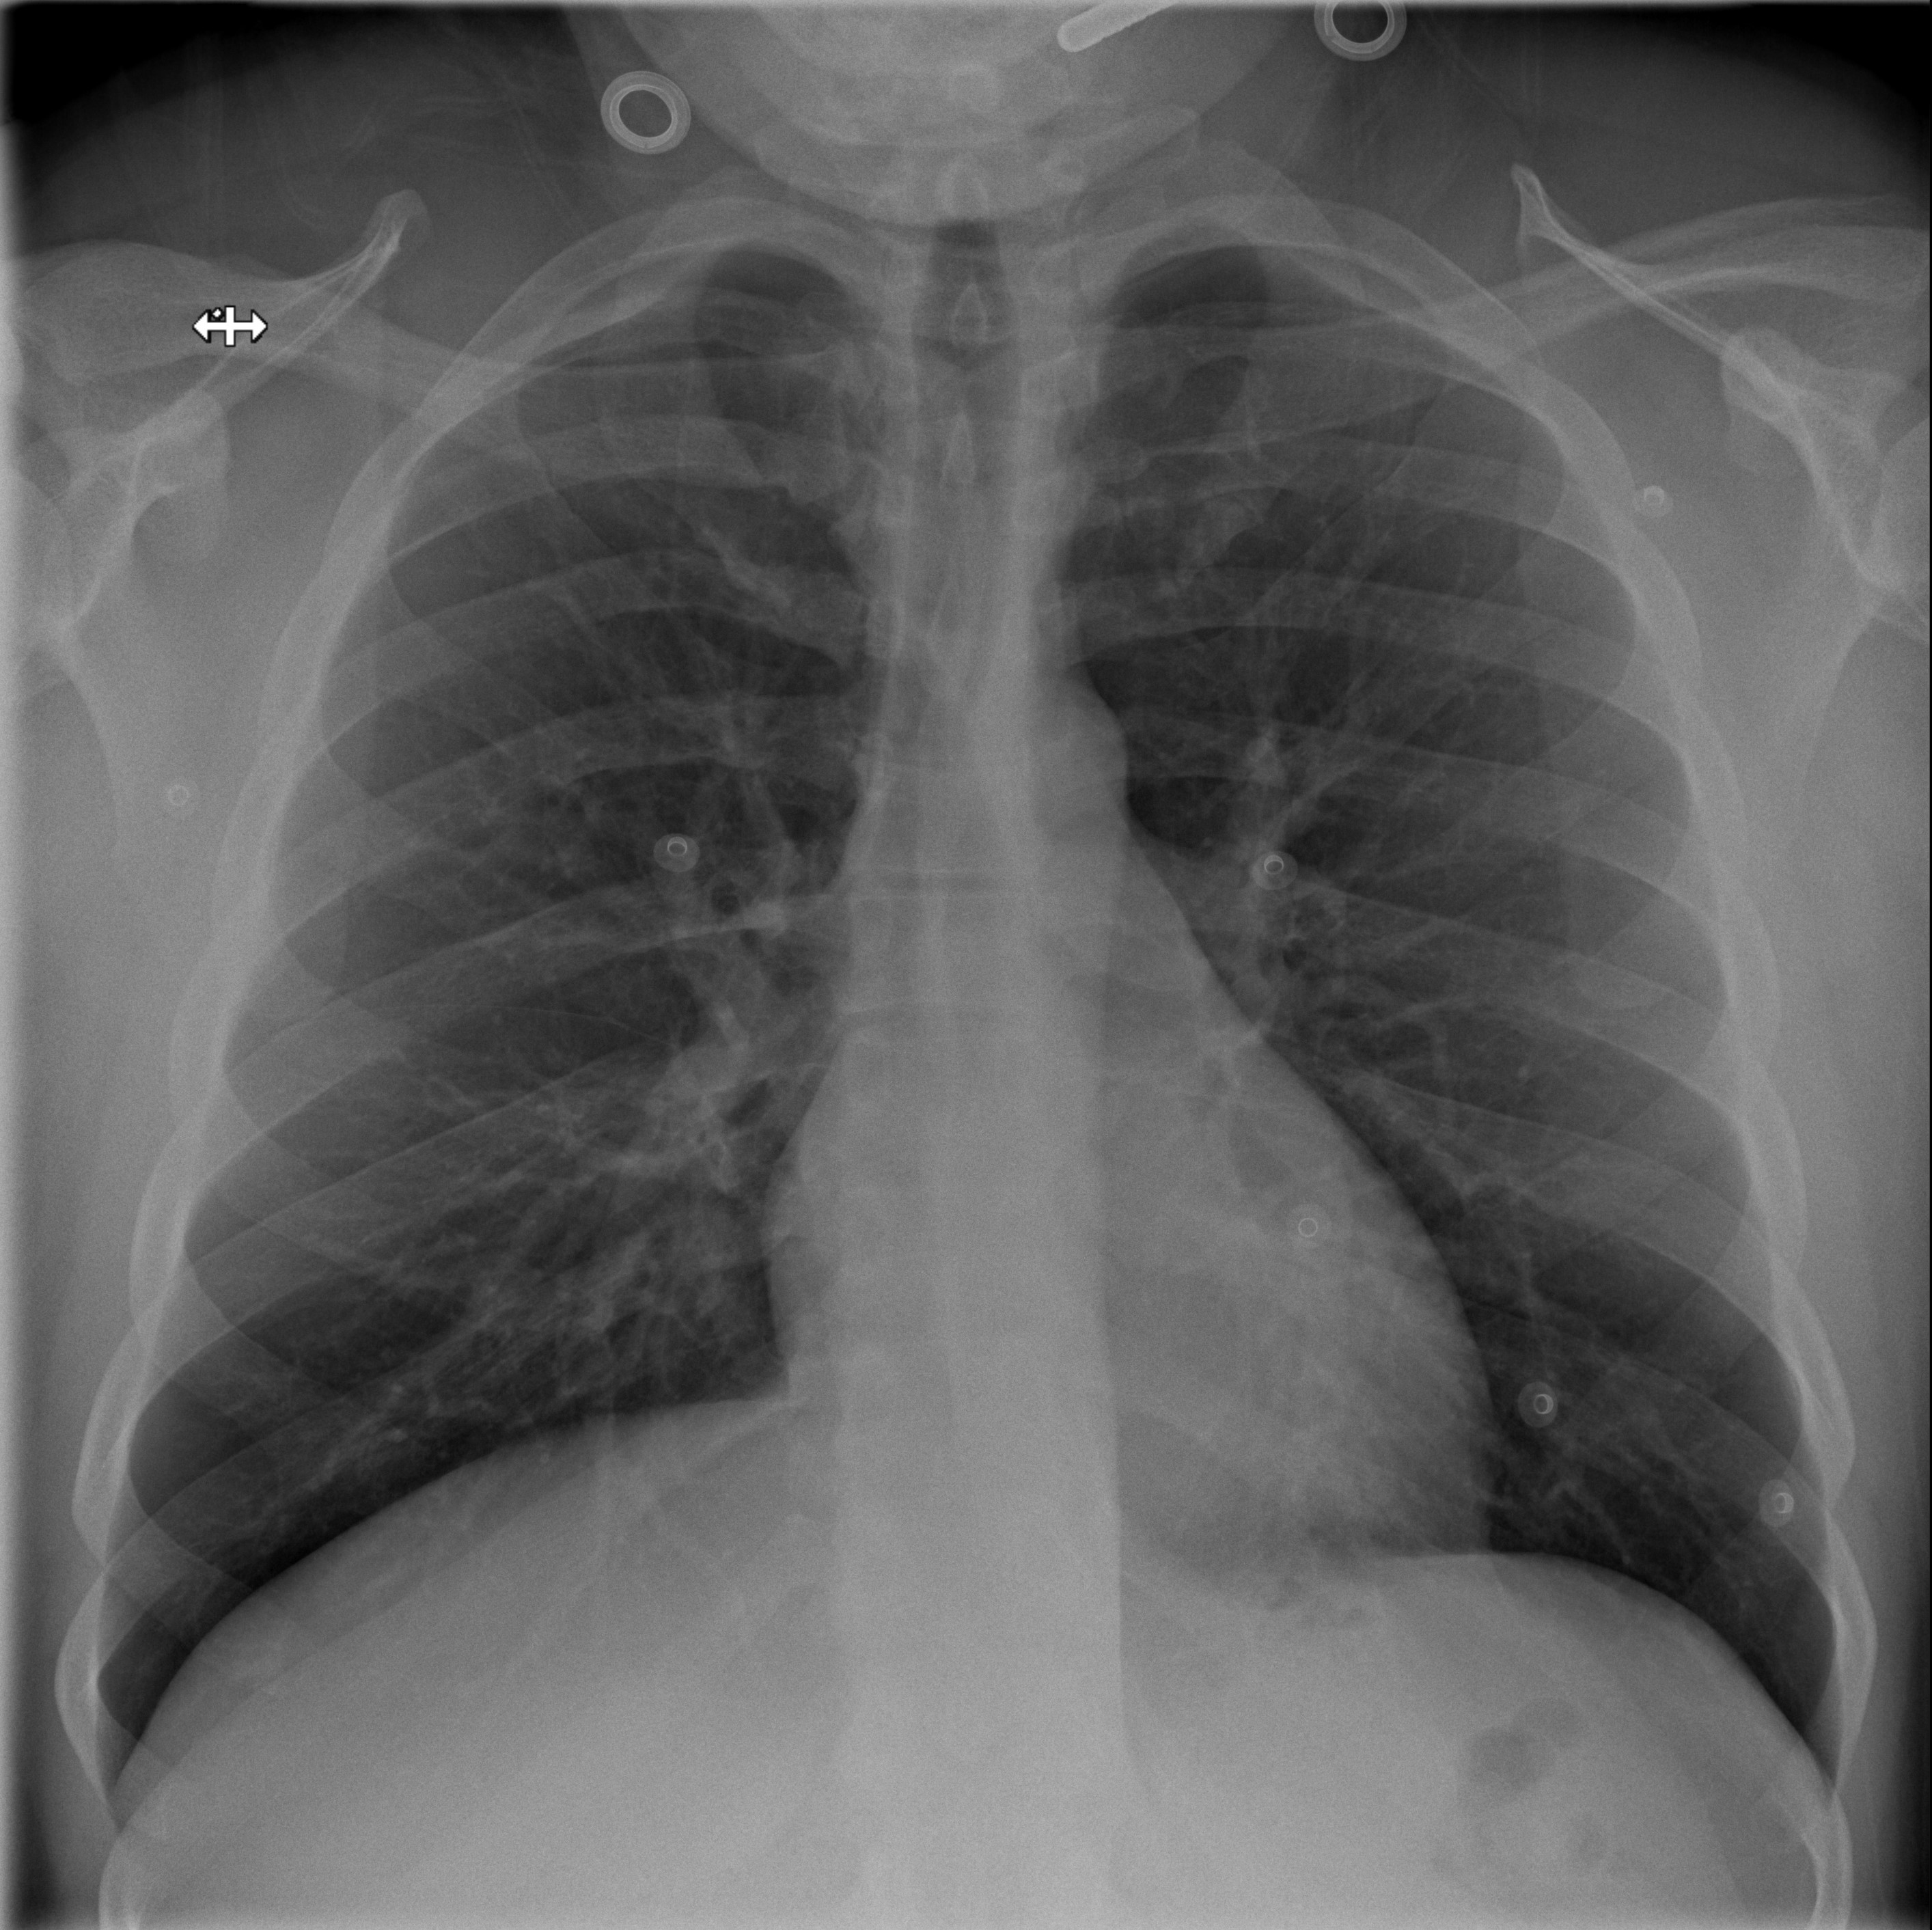
\includegraphics[width=.95\linewidth]{P_1_10.png}  
        \caption{MILD}
        %\label{MILD}
        %MILD
    \end{subfigure}
    \begin{subfigure}{.45\textwidth}
        \centering
        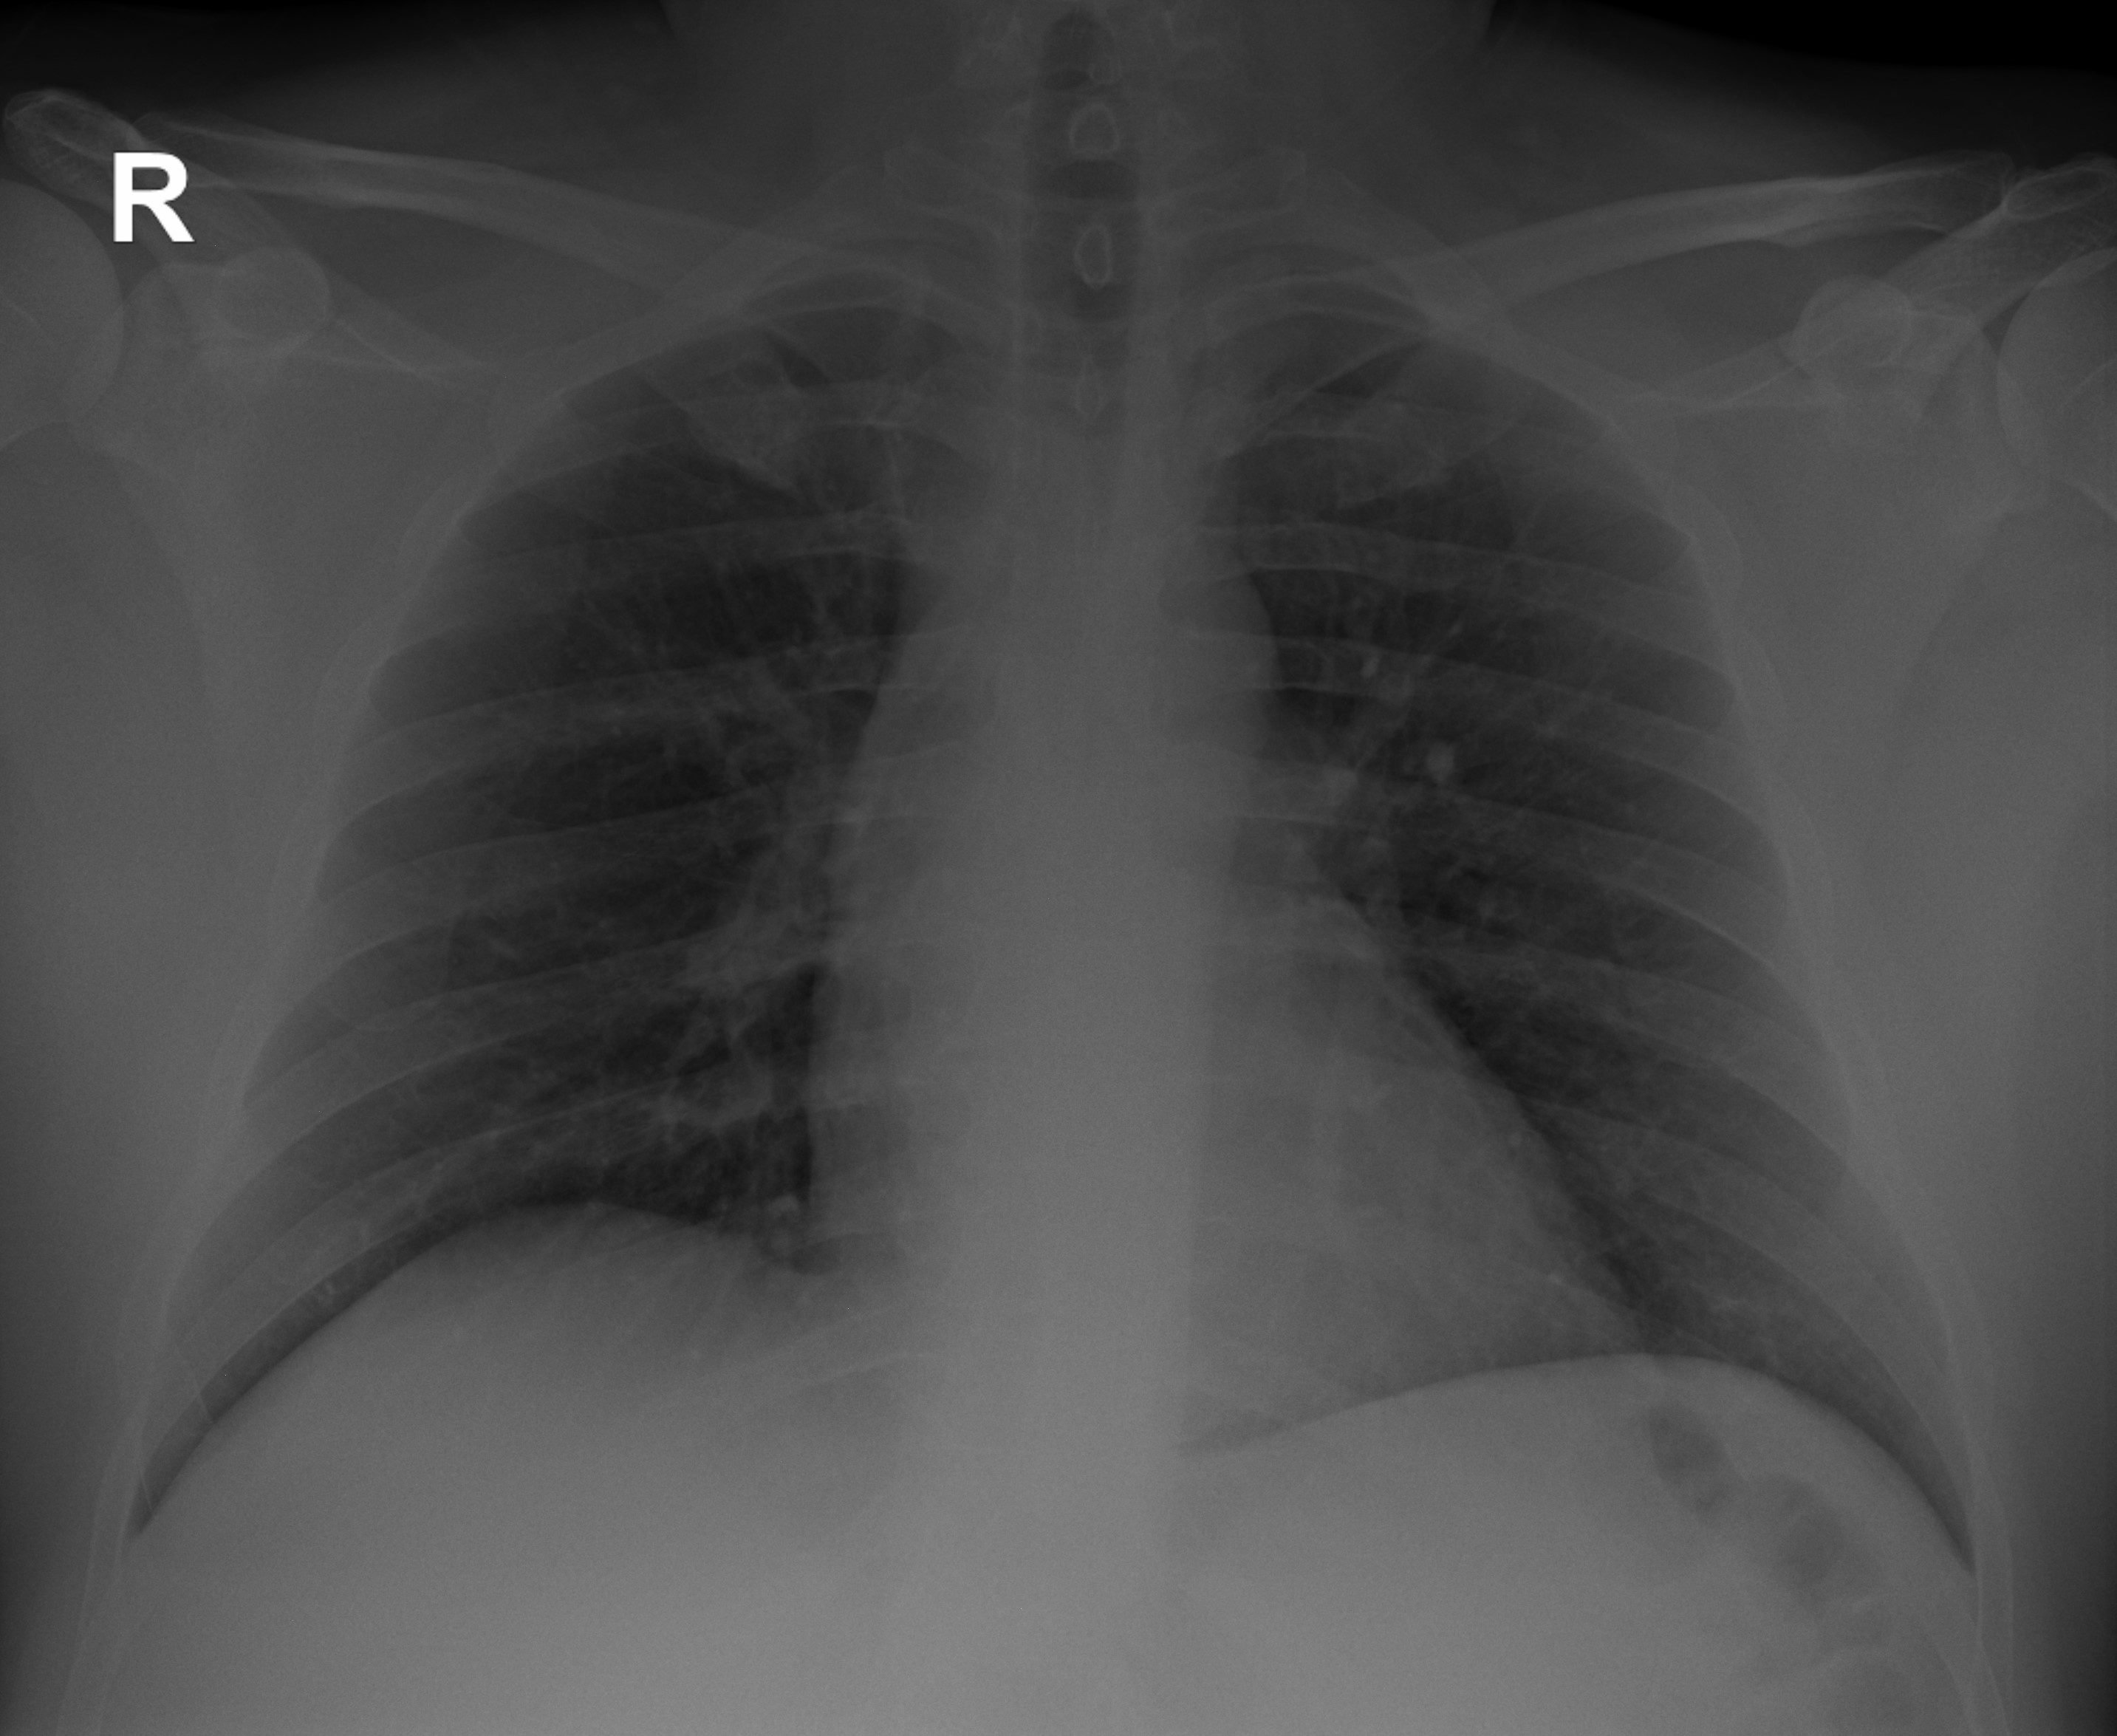
\includegraphics[width=.95\linewidth]{P_2_27.png}  
        \caption{MILD}
        %\label{MILD}
        %MILD
    \end{subfigure}
    \begin{subfigure}{.45\textwidth}
        \centering
        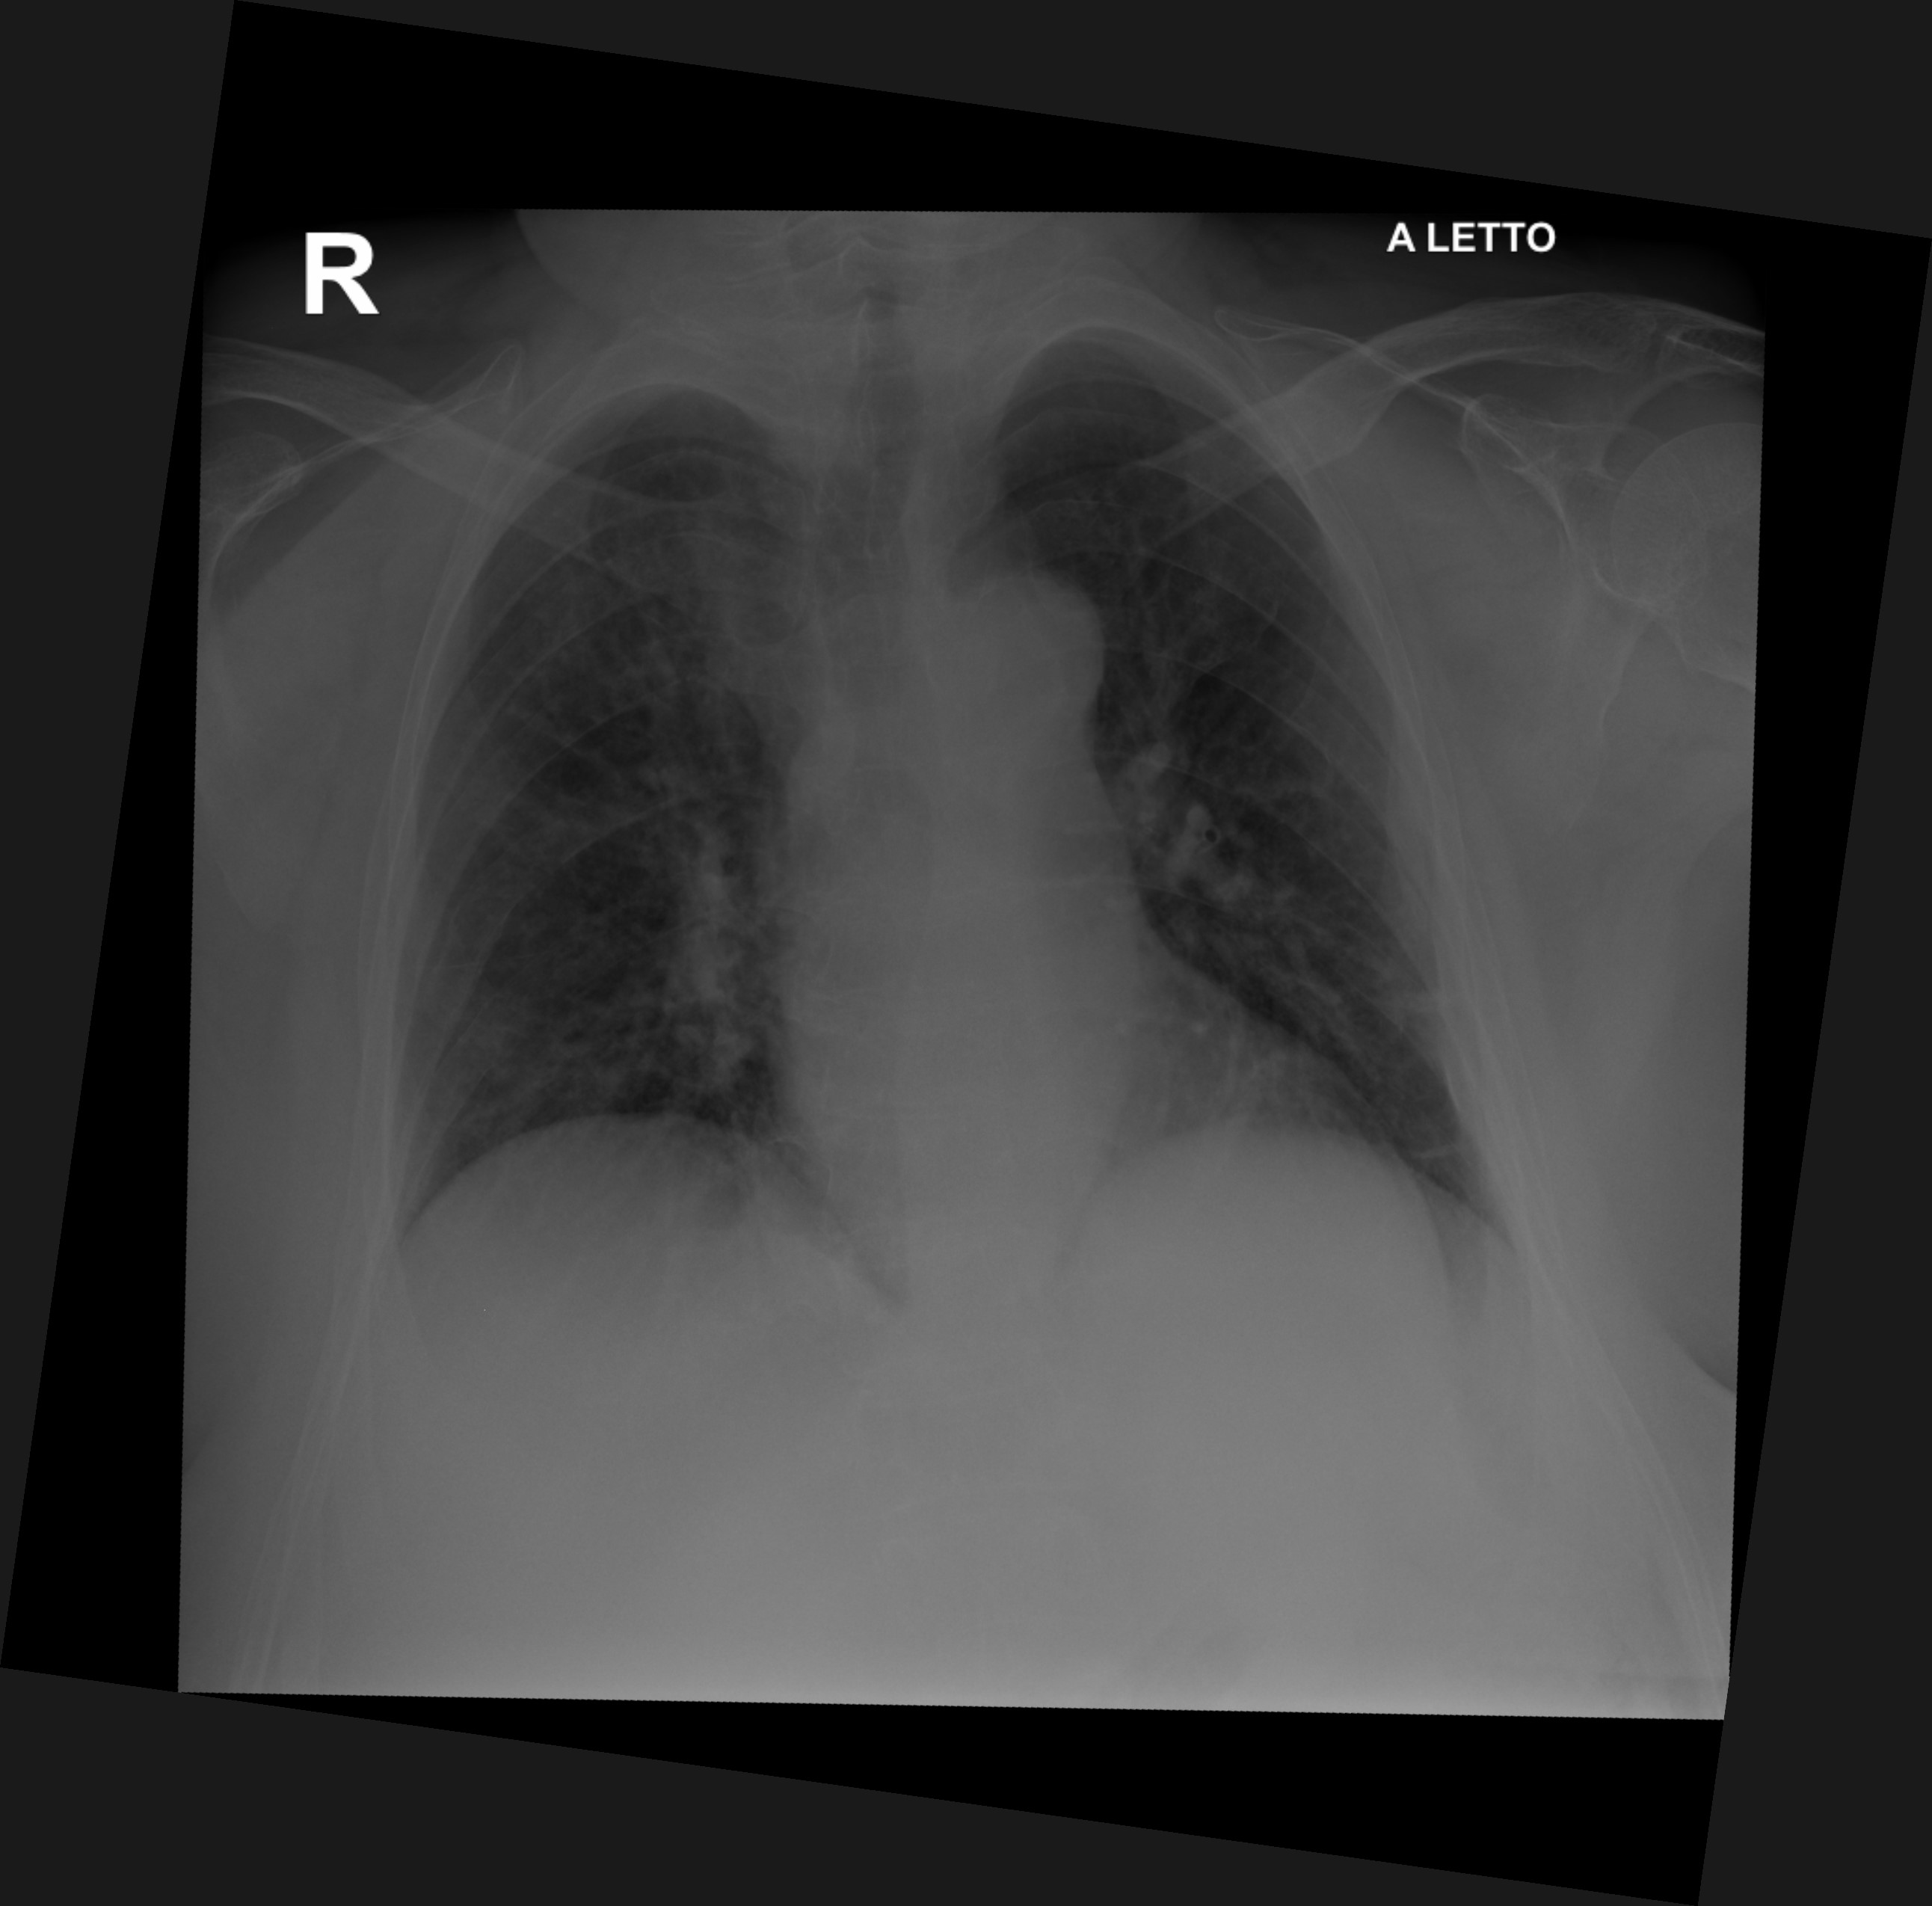
\includegraphics[width=.95\linewidth]{P_2_68.png}  
        \caption{SEVERE}
        %\label{SEVERE}
        %SEVERE
    \end{subfigure}
    \begin{subfigure}{.45\textwidth}
        \centering
        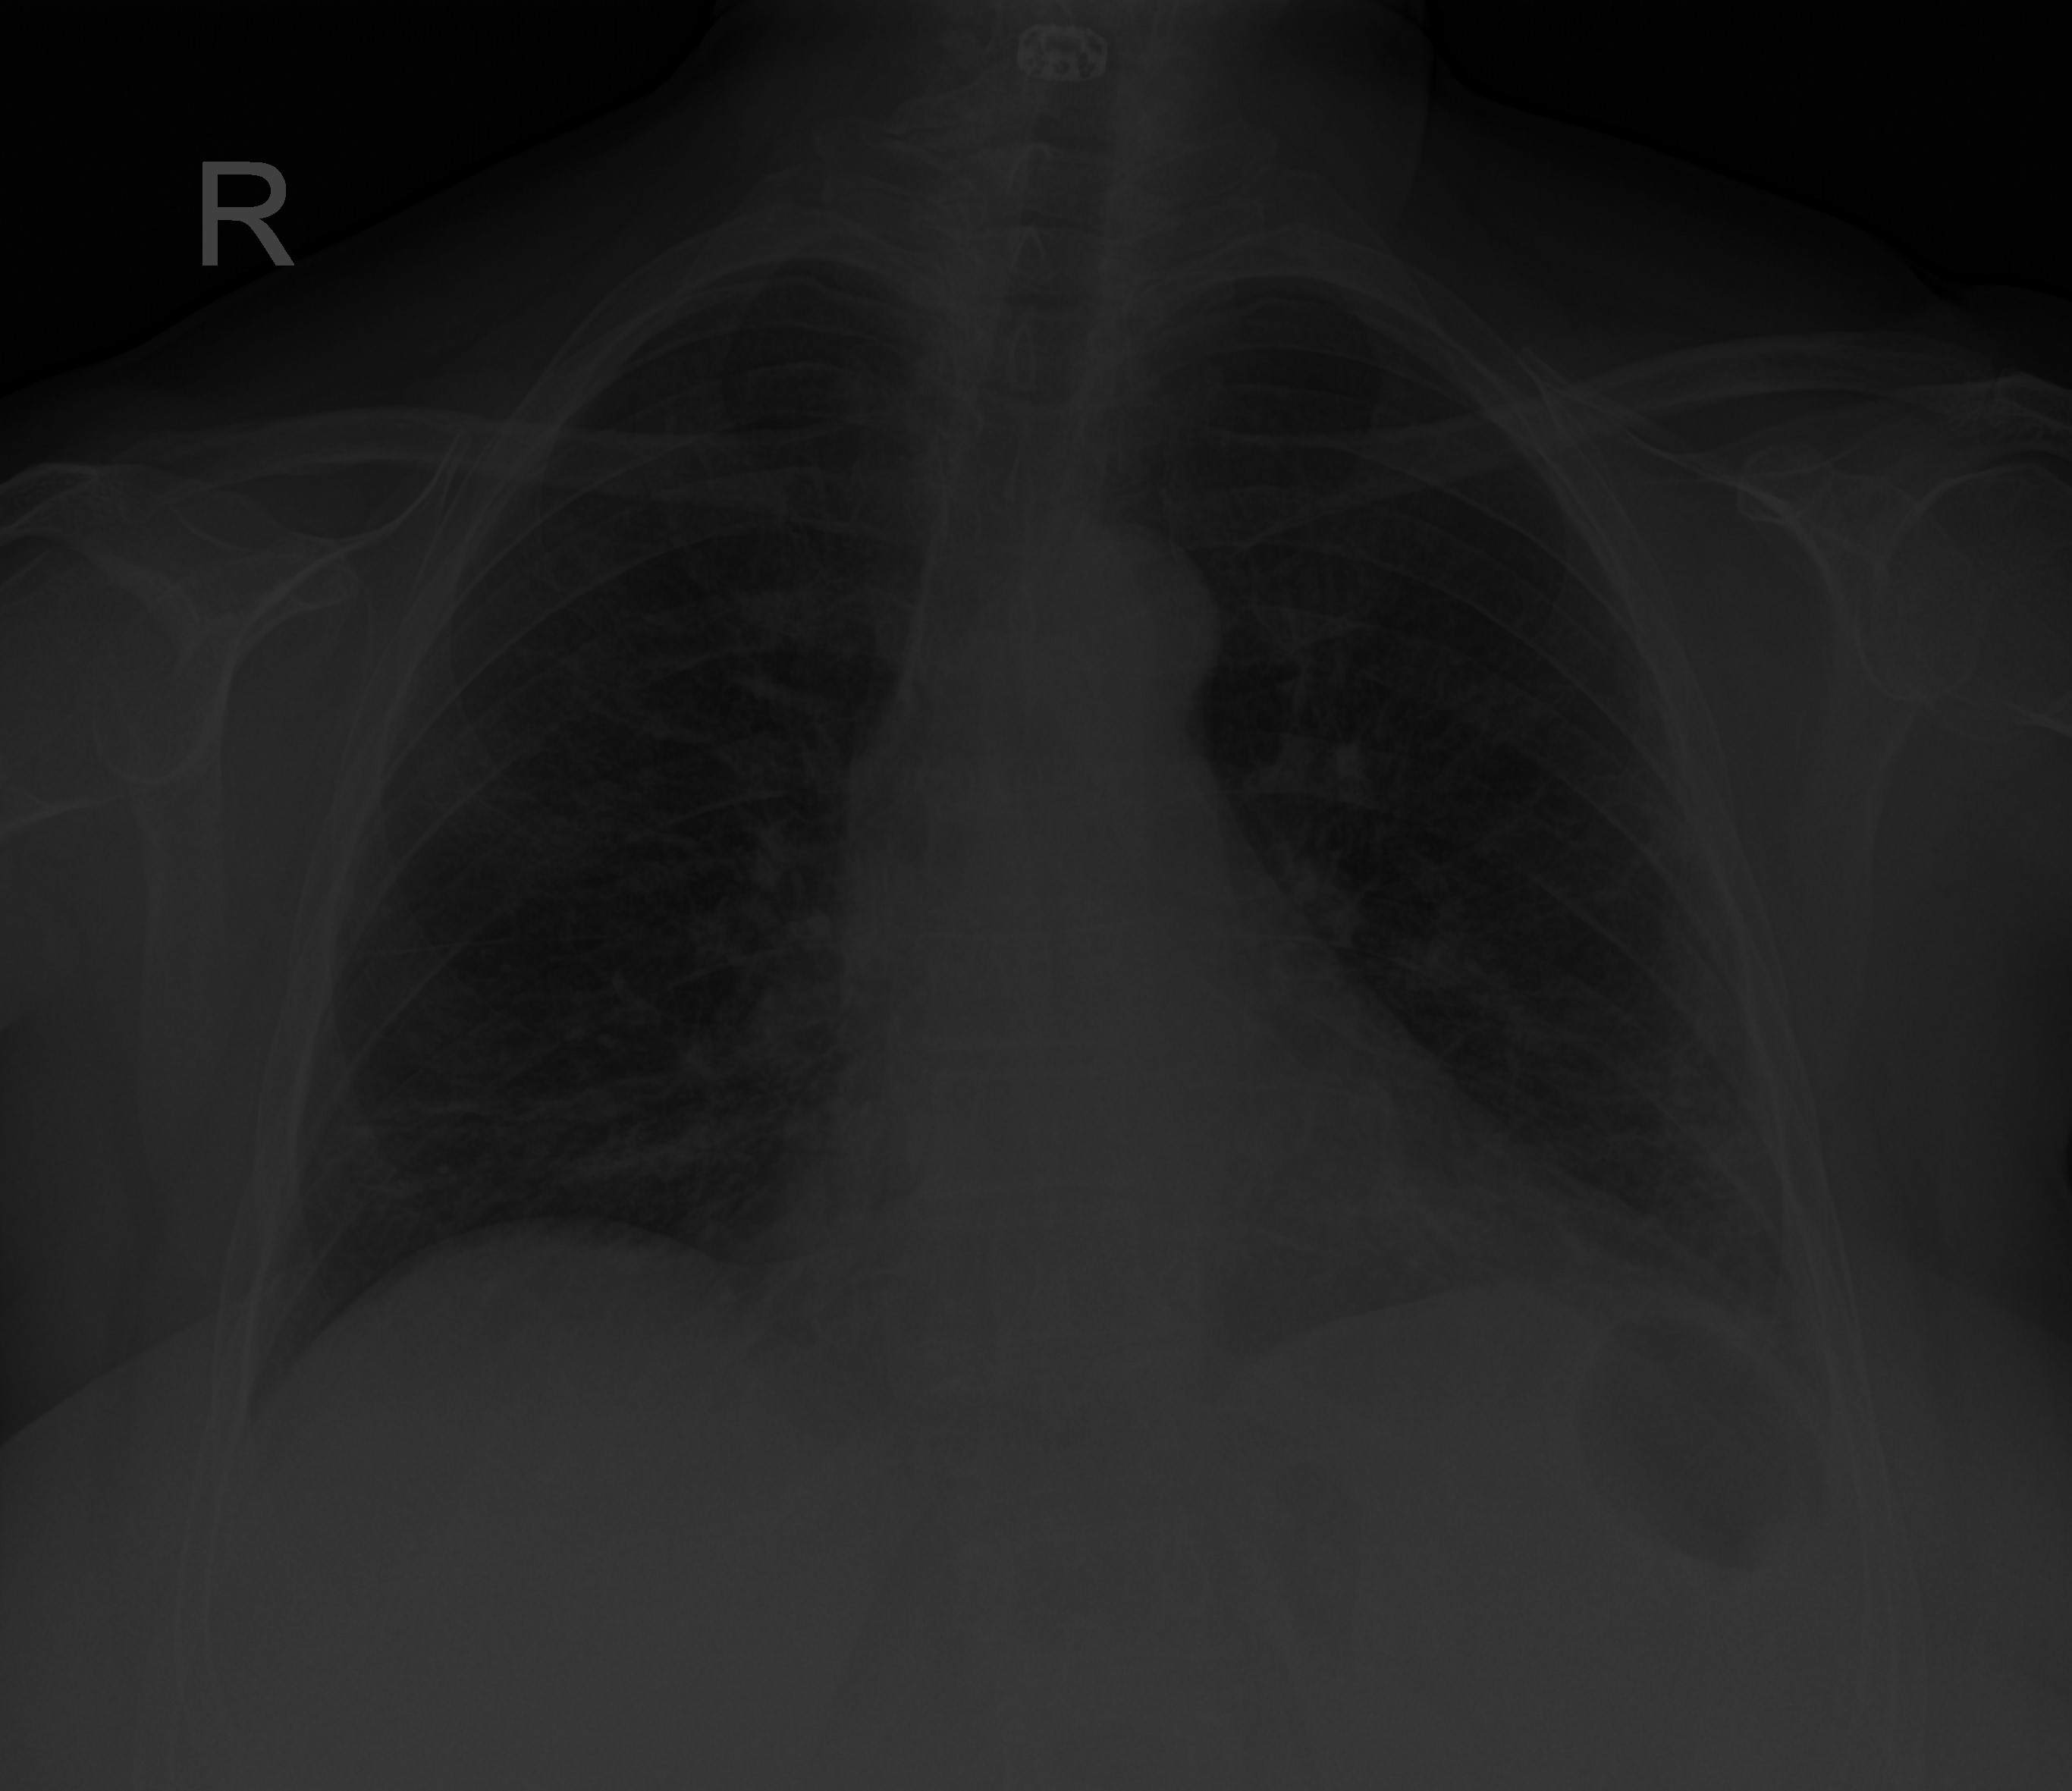
\includegraphics[width=.95\linewidth]{P_163.png}  
        \caption{SEVERE}
        %\label{SEVERE}
        %SEVERE
    \end{subfigure}
    \caption{Campione del dataset per evidenziare le differenze tra le immagini}
    \label{Campione}
\end{figure}
$\\\\$
Oltre alla differenza nelle dimensioni delle varie immagini si possono notare diversità relative a luminosità, contrasto ed alcune sono in negativo.
Per tali motivi risulta utile eseguire un preprocessing delle immagini, in cui si effetuano vari passaggi:
\begin{itemize}
    \item Regolare contrasto, luminosità ed effettuare un check sulle immagini in negativo,
    \item Riconoscere i polmoni e crearne una mascehera,
    \item Ricavare una bounding-box che contenga i polmoni,
    \item Ritagliare la bounding-box contenente i polmoni, in modo che abbiano tutte la stessa dimensione.
\end{itemize}

È importante sottolineare che nell'eseguire tali passaggi si necessita di evitare di distorcere l'immagine, per tale 
motivo si faranno considerazioni sull'aspect ratio dell'immagine.
\\\\
Per prima cosa si sfrutta la libreria OpenCV \cite{ocv} al fine di normalizzare il contrasto dell'immagine mediante la funzione convertScaleAbs() ed 
equalizzare l'istogramma, mediante l'uso di CLAHE (Contrast Limited Adaptive Histogram Equalization) in modo anche da correggere la luminosità.
convertScaleAbs() è una funzione che svolge varie operazioni in sequenza:
\begin{itemize}
    \item effettua un rescaling basato sul fattore passato come argomento, nel caso in questione 1 (non effettuiamo rescaling),
    \item aggiunge un offset passato come secondo parametro, nel caso considerato tale offset è impostato a 0,
    \item calcola il valore assoluto della somma ottenuta dal passaggio precedente.
\end{itemize}
L'uso del CLAHE è dovuto al fatto che immagini di buona qualità hanno pixel in tutte le regioni dell'immagine, per tale motivo si necessita di 
allungare l'istogramma dell'immagine alle estremità. Tale operazione è detta equalizzazione dell'istogramma. In alcune immagini, come quelle più luminose, 
i pixel sonon invece confinati in una sola estremità dell'istogramma. L'istogramma di un'immagine rappresenta la distribuzione dei colori all'interno dell'immagine.
Quello che si vuole dunque ottenere è un istogramma più piatto possibile, ovvero far si che tutti i colori abbiano la stessa distribuzione nell'immagine.
Tale operazione ha come conseguenza il miglioramento del contrasto dell'immagine, per questo risulta essere utile.
\\\\
Si è notato inoltre che alcune immagini del dataset risultavano essere in negativo, ovvero erano più luminose sullo sfondo e meno luminose al centro (dove si trovano i polmoni).
Per affrontare tale problematica si è deciso di prendere un campione di pixel alle estremità dell'immagine e confrontarlo con uno preso al centro.
Tale confronto viene effettuato calcolando una soglia, facendo la media dei colori dei pixel dell'immagine.
Se il campione supera tale soglia indica che il campione è più luminoso. Poi si calcola la percentuale di bianco in entrambi i campioni. 
Se la percentuale di bianco presente nel campione relativo agli angoli risulta essere maggiore di quella presente nel campione preso dal centro dell'immagine, allora 
l'immagine è in negativo e per tale motivo si riporta l'immagine allo stato originale sottroendo  i valori dei pixel attuali ad un'immagine completamente nera.
In tal modo si è riportata l'immagine "in positivo".
\\\\
Tali passaggi serviranno per ottenere immagini omogenee, in grado di consentire alla rete di identificare i polmoni.
\section{Utilizzo di una rete convoluzionale per segmentazione delle immagini}
Al fine di effettuare il riconoscimento dei polmoni all'interno dell'immagine, si sfrutta una U-Net.
Una U-Net è una rete convoluzionale sviluppata per eseguire la segmentazione dell'immagine. Il processo di segmentazione consiste nell'assegnare ad 
ogni gruppo di pixel selezionato una categoria. Ad esempio si potrebbe avere un insieme di pixel del'immagine che identificano il contorno dei polmoni.
\\\\
Lo scopo della U-Net è dunque quello di prendere in input l'immagine e creare una maschera che raffiguri i polmoni.
La maschera è un'immagine formata da pixel con valore in [0,1] e mira a creare un'immagine raffigurante la distinzione tra cosa rappresenta 
i polmoni e cosa rappresenta lo sfondo.
L'utilià della maschera è quella di consentirci di trovare con maggior facilità la bounding box.
\\\\
La rete usata per la segmentazione è EfficientNet. Tale rete prende un input di dimensione predefinita e restituisce un'immagine della stessa
dimensione, rappresentante la maschera. Nel caso considerato, inoltre si è deciso di usare come funzione di attivazione Sigmoid e di sfruttare 
i pesi preallenati su ImageNet, per avere maggior precisione.
\\\\
Essendo le immagini di dimensione diversa, prima di darle in input alla rete viene effettuato un ridimensionamento alle dimensioni accettate dalla rete. 
Tale passaggio viene effettuato mantenendo l'aspect ratio dell'immagine e inserendo padding nero per evitare distorsione.
L'aspect ratio rappresenta il rapporto tra le dimensioni dell'immagine, per evitare distorsione della stessa, si deve conseravre tale rapporto.
Nel caso in cui l'immagine non soddisfi i requisiti delle nuove dimensioni si procede con l'aggiunta di padding di colore nero, ovvero si inseriscono i pixel necessari 
all'immagine per raggiungere la dimensione necessaria usando un colore non influente. 
\\\\
La rete performa molto bene con immagini di dimensioni piccole, tuttavia si è potuto notare, a seguito di esperimenti, che nel caso considerato, la rete 
performa meglio con immagini, in input, di dimensione 256 x 256 rispetto a quelle di dimensione 224 x 224.
Per tale motivo, a seguito della segmentazione dovrà essere effettuato un ridimensionamento dell'immagine.

\section{Selezione delle sezioni di interesse nelle immagini}
Ottenute così le maschere retive alle immagini, queste sono alla base della costruzione delle bounding-box.
La bounding-box rappresenta il riquadro di dimensione minima, contenente i polmoni.
Per trovare tale riquadro si usano i punti estremi delle maschere: si cercano il punto più alto, più basso, il più a destra e l'estremo a sinistra.
Tali punti rappresentano le coordinate di una box, la quale conterrà per certo i polmoni.
\\\\
Avendo ora le bounding box, l'ultima cosa da fare è ritagliare le dalle immagini originali le bounding-box e ridimensionarle a 224 x 224.
È necessario in questi passaggi di ridimensionamento mantenere presente che l'aspect-ratio deve essere conservato, per cui si effettua nuovamente padding ove necessario.
\\\\
Alla fine di tale procedimento si sono ottenute delle immagini raffiguranti i polmoni e della dimensione desiderata.
\begin{figure}[h]
    \centering
    \begin{subfigure}{.45\textwidth}
        \centering
        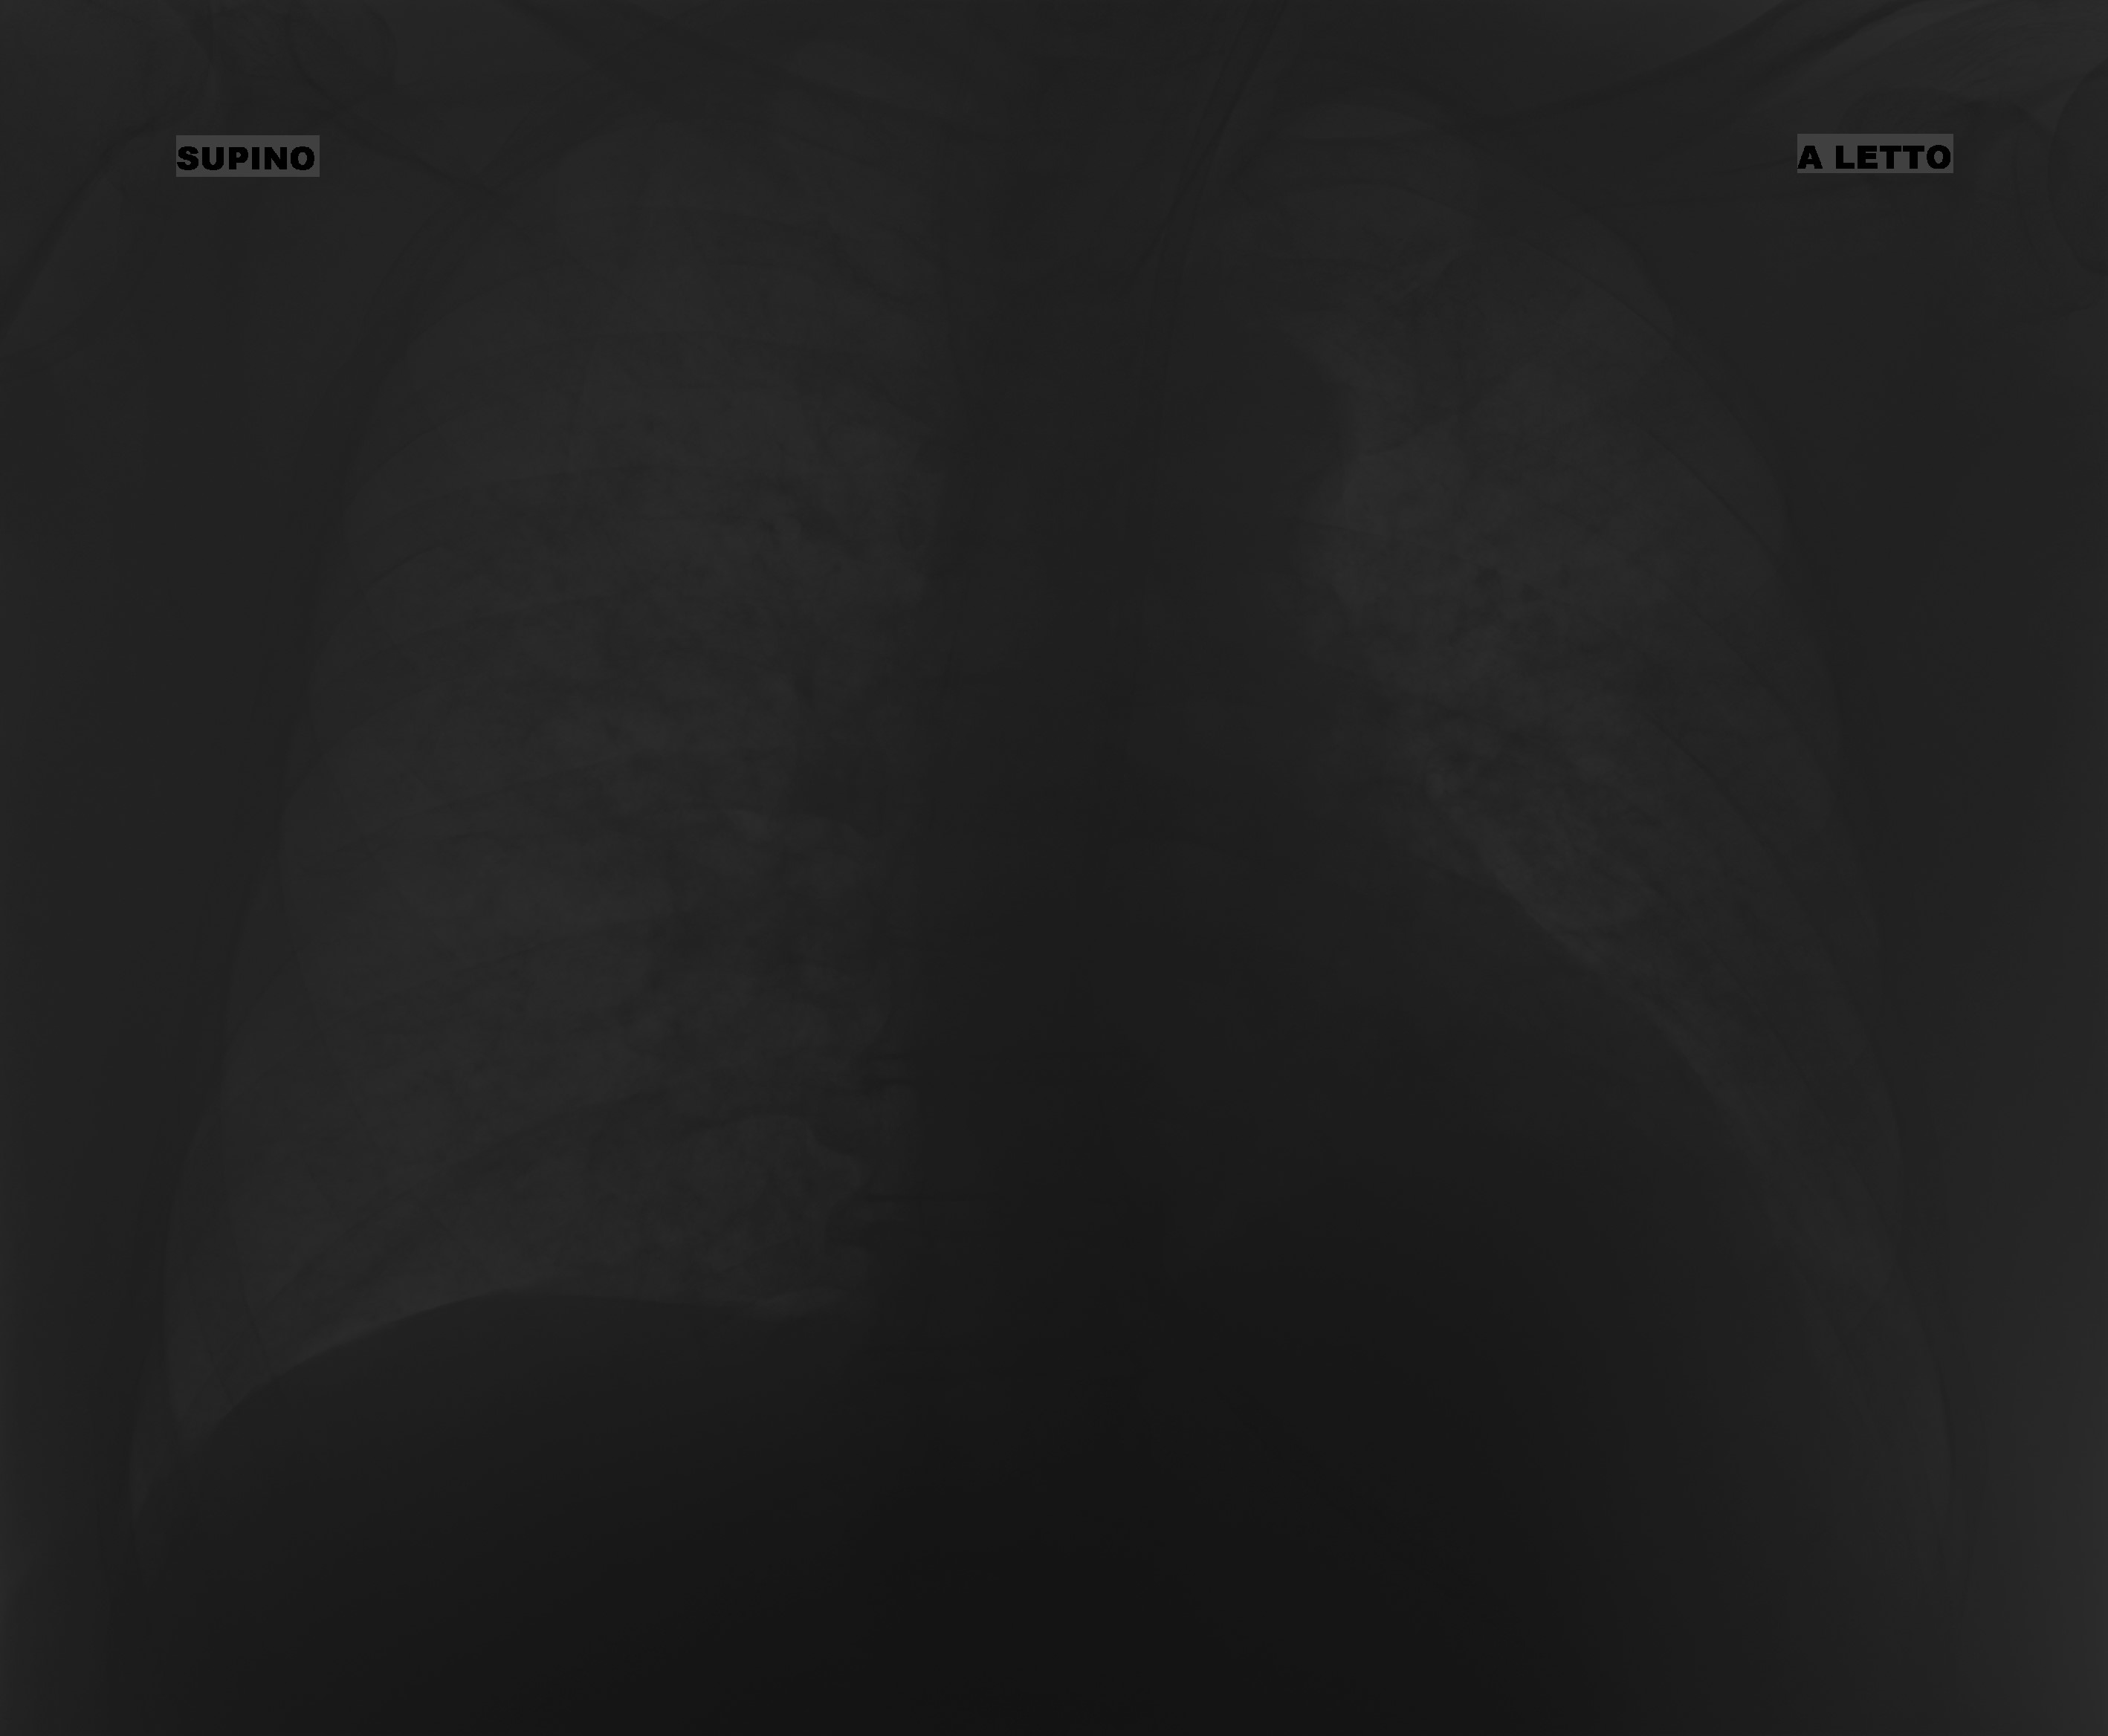
\includegraphics[width=.95\linewidth]{P_1_11_or.png}  
        \caption{Immagine originale}
        %\label{SUBFIGURE LABEL 1}
    \end{subfigure}
    \begin{subfigure}{.45\textwidth}
        \centering
        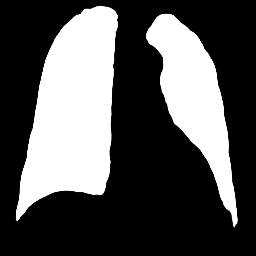
\includegraphics[width=.95\linewidth]{P_1_11_mask.png}  
        \caption{Maschera creata dalla U-Net}
        %\label{SUBFIGURE LABEL 2}
    \end{subfigure}
    \begin{subfigure}{.45\textwidth}
        \centering
        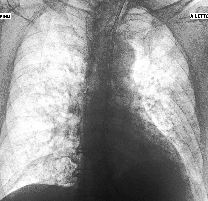
\includegraphics[width=.95\linewidth]{P_1_11.png}  
        \caption{Immagine finale}
        %\label{SUBFIGURE LABEL 3}
    \end{subfigure}
    \caption{Effetti dei vari passaggi sulle immagini del dataset}
    \label{Transformation}
\end{figure}
\section{Metadati relativi alle radiografie dei pazienti}
Per quanto riguarda i metadati la situazione è meno complessa, poichè gestita mediante file csv.
Il dataset in questo caso è sempre diviso in training e test set, ma è composto da un insieme di righe e colonne:
le righe rappresentano i vari pazienti, mentre le colonne rappresentano vari dati relativi al paziente.
\\\\
\phantomsection \label{eterogeneo}Le colonne iniziali di tali dataset sono le stesse e sono: 
    ospedale,
    età,
    sesso, 
    positività all'ammssione, 
    temperatura corporea,
    giorni di febbre, 
    tosse,
    difficoltà respiratorie,
    WBC,
    RBC,
    CRP,
    fibrina, 
    glucosio, 
    PCT, 
    LDH, 
    INR, 
    D\_dimer, 
    percentuale di ossigeno, 
    PaO2, 
    SaO2, 
    PaCO2, 
    pH, 
    malattie cardiovascolari,
    cardiopatia ischemica,
    fibirllazione atriale,
    insufficienza respiratoria,
    arresto cardiaco,
    ictus,
    alta pressione sanguigna,
    diabete,
    demenza,
    BPCO,
    cancro,
    malattia renale cronica,
    insufficienza respiratoria,
    obesità,
    posizione.
\\\\
Questi rappresentano i dati, oltre a tali colonne sono presenti una colonna che rappresenta un identificativo del paziente, una colonna col nome 
del file contenente la radiografia dei polmoni e una colonna contenente la prognosi (vuota nel caso del test set).
\\\\
\begin{tcolorbox}[tab2,tabularx={Y|Y|Y|Y|Y|Y|Y|Y|Y|Y},title=Estratto del dataset di training,width=\textwidth, center=\textwidth]
    \centering
    \begin{tabular}{l|l|c|c|c|c|c|c|l}
        ImageFile & H. & Age & Sex & ...... & T.C. & D.F. & Diabetes & Prognosis \\ \hline \hline
        ... & ... & ... & ... & ... & ... & ... & ... & ... \\
        P\_601.png & B & 68 & 0 &...& 38 & 3 & 0 & SEVERE \\
        
        P\_402.png & F & 74 & 1 &...& 36 & 3 & 0 & MILD \\
        
        P\_72.png & A & 72 & 1 &...& 36.1 & 3 & 0 & MILD  \\
        
        P\_608.png & B & 38 & 1 &...& 37.5 & 3 & 0 & MILD  \\
        
        P\_396.png & F & 63 & 1 &...& 36 & 3 & 0 & MILD \\
        ... & ... & ... & ... & ... & ... & ... & ... & ... 
    \end{tabular}     
\end{tcolorbox}
\begin{tcolorbox}[tab2,tabularx={Y|Y|Y|Y|Y|Y|Y|Y|Y|Y},title=Estratto del dataset di test,width=\textwidth, center=\textwidth]
    \centering
    \begin{tabular}{l|l|c|c|c|c|c|c|l}
        ImageFile & H. & Age & Sex & ...... &  T.C. & D.F. & Diab. & Prognosis \\ \hline \hline 
        ... & ... & ... & ... & ... & ... & ... & ... & ... \\
        P\_3\_428.png & F & 78 & 1 &... & 35.8 & 1 & 0 & nan \\ 

        P\_3\_158.png & F & 65 & 1 &... & 36.6 & 3 & 0 & nan\\  

        P\_3\_429.png & F & 45 & 0 &... & 38 & 4 & 0 & nan \\

        P\_3\_299.png & F & 80 & 0 &... & 38.4 & 3 & 0 & nan \\

        P\_3\_483.png & F & 63 & 0 &...& 36 & 1 & 1 & nan \\
        ... & ... & ... & ... & ... & ... & ... & ... & ... 
    \end{tabular}     
\end{tcolorbox}
$\\\\$
Ciò che si vuole ottenere, al fine di usare tali metadati insieme alle immagini per effettuare il training, è un insieme di dati che sia completamente pieno, ovvero presenti corrispondenze 
per tutte le righe e colonne del dataset.
\\\\
Dunque si cerca di ridurre il dataset di partenza nel più grande sottinsieme che contenga tutte le corrispondenze.
Tale omogeneità deve essere presente sia nel dataset di training che in quello di test. Oltre a ciò, alla fine, si cerceranno le collonne comuni 
ai due dataset, scartando le altre. In tal modo si possono unire i due dataset così da formarne uno solo.
\\\\ 
Per iniziare si eliminano le colonne che non presentano alcun dato, o che presentano dati solo per un numero molto ristretto di paziente, per :
\begin{itemize}
    \item nel dataset di training sono state scartate le colonne:
        giorni di febbre, 
        fibrina, 
        glucosio, 
        PCT, 
        LDH, 
        INR, 
        D\_dimer, 
        percentuale di ossigeno, 
        PaO2, 
        SaO2, 
        PaCO2, 
        pH, 
        cardiopatia ischemica,
        insufficienza respiratoria,
        obesità, 
        positività all'ammssione, 
        temperatura corporea, 
        RBC, 
        CRP.
    \item nel dataset di test sono state scartate le colonne:
    giorni febbre, 
    fibrina, 
    LDH,
    PaO2,
    PaCo2, 
    pH, 
    PCT, 
    INR,
    D\_dimer, 
    SaO2, 
    tempertaure corporea, 
    CRP. 
\end{itemize} 
$\\\\$
Eliminate le colonne in eccesso, si procede con l'eliminazione dei paziente che non presentano tutti i dati.
A seguito di tale operazione le righe, ovvero i pazienti, che sono presenti nel dataset di train sono 946, mentre quelle del dataset di test
472.
Le colonne in comune tra i due dataset sono:
\begin{itemize}
    \item Ospedale, 
    \item Età, 
    \item Sesso,
    \item Tosse, 
    \item Difficoltà respiratorie
    \item Numero di cellule bianche,
    \item Pressione sanguigna alta,  
    \item Diabete,
    \item Demenza,  
    \item BPCO (Broncopneumopatia cronica ostruttiva),
    \item Cancro, 
    \item Malattia renale cronica
\end{itemize}
$\\\\$
In tal modo si è ottenuto un dataset che contiene 12 colonne significativa (sopra elencate) contenenti dati per 
1418 pazienti.
$\\\\$
\begin{tcolorbox}[tab2,tabularx={Y|Y|Y|Y|Y|Y|Y|Y|Y|Y},title=\text{Estratto del dataset di training, in seguito alle modifiche},width=\textwidth, center=\textwidth]
    \centering
    \begin{tabular}{l|c|c|c|c|c|c|c|c|l}
        ImageFile & H. & Age & Sex & ...... & C. & WBC & Ic. & Canc. & Prognosis \\ \hline \hline
        ... & ... & ... & ... & ... & ... & ... & ... & ... & ...\\
        P\_134.png & D & 53 & 1 &... & 0 & 6.92 & 0 & 0 & MILD  \\
        P\_761.png & F & 42 & 1 &... & 0 & 4 & 0  & 0 & MILD  \\
        P\_337.png & E & 56 & 0 &... & 0 & 3.37 & 0 & 0 & SEVERE  \\
        P\_288.png & E & 71 & 0 &... & 0 & 6.96 & 1 & 0 & MILD  \\
        P\_429.png & F & 86 & 1 & ...& 1 & 4.3 & 0 & 1 & SEVERE \\
        ... & ... & ... & ... & ... & ... & ... & ... & ... & ...\\
    \end{tabular}     
\end{tcolorbox}

\begin{tcolorbox}[tab2,tabularx={Y|Y|Y|Y|Y|Y|Y|Y|Y|Y|Y},title=\text{Estratto del dataset di test, in seguito alle modifiche}, width=\textwidth, center=\textwidth]
    \centering
    \begin{tabular}{l|c|c|c|c|c|c|c|c|l}
        ImageFile & H. & Age & Sex & ...... & C. & WBC & RBC & G. & Diab.   \\ \hline \hline
        ... & ... & ... & ... & ... & ... & ... & ... & ... & ...\\
        P\_3\_455.png & F & 47 & 0 &...& 0 & 9.29 & 5.18 & 99  & 0  \\
        P\_3\_342.png & F & 33 & 0 &... & 1  & 4.65 & 4.65 & 101  & 0   \\
        P\_3\_96.png & F & 62 & 1 &... & 0  & 8.3 & 4.35 & 157 & 0   \\
        P\_3\_6.png & F & 49 & 1 &... & 1  & 8.16 & 4.84 & 243 & 0   \\
        P\_3\_22.png & F & 52 & 0 &... & 1  & 3.5 & 5.32 & 147  & 0  \\
        ... & ... & ... & ... & ... & ... & ... & ... & ... & ...
    \end{tabular}     
\end{tcolorbox}